%!TEX root = ./template-skripsi.tex
%-------------------------------------------------------------------------------
%                            BAB II
%               KAJIAN TEORI
%-------------------------------------------------------------------------------

\chapter{KAJIAN PUSTAKA}                
	
\section{Monitoring dan Evaluasi}

	Monitoring adalah sebuah kegiatan mengamati secara seksama suatu keadaan atau kondisi, termasuk perilaku atau kegiatan tertentu, dengan tujuan agar semua data atau informasi masukan yang didapat dari hasil pengamatan tersebut dapat dijadikan landasan dalam pengambilan keputusan tindakan yang perlu dilakukan selanjutnya. 

	Tindakan tersebut diperlukan seandainya dari hasil pengamatan didapatkan adanya hal atau kondisi yang tidak sesuai dengan rencana atau aturan yang dibuat sebelumnya. Monitoring dilaksanakan dengan maksud agar kegiatan yang dilakukan dapat mencapai tujuan yang diinginkan secara efektif dan efisien.

	Proses dasar dalam monitoring meliputi tiga tahap, yaitu menetapkan standar pelaksanaan, pengukuran pelaksanaan, dan menentukan perbedaan antara pelaksanaan dengan aturan dan rencana awal. Monitoring memiliki empat fungsi, yaitu: \citep{Dunn2014}
\begin{itemize}
	\item Ketaatan (compliance). Monitoring menentukan apakah tindakan setiap bagian anggota yang terlibat sesuai dengan norma, nilai, dan standar yang ditetapkan dalam menjalankan tugasnya.
	\item Pemeriksaan (auditing). Monitoring menetapkan apakah fasilitas dan layanan yang diperuntukkan bagi suatu pihak benar-benar tersampaikan dengan baik.
	\item Laporan (accounting). Monitoring menghasilkan informasi dan data untuk membantu melihat hasil perubahan sosial sebagai akibat implementasi keputusan sesudah beberapa periode waktu.
	\item Penjelasan (explanation). Monitoring menghasilkan informasi yang dapat membantu menjelaskan bagaimana efek diterapkannya sebuah kebijakan dan menjelaskan alasan kecocokan perencanaan dan pelaksanaannya.
\end{itemize}
	Monitoring dan evaluasi memiliki kaitan yang sangat erat, karena dalam evaluasi dibutuhkan hasil monitoring untuk melihat pengaruh dari program yang berjalan.

	Evaluasi merupakan proses yang sistematis dan berkelanjutan untuk mengumpulkan, mendeskripsikan, menginterpretasikan, dan menyajikan informasi untuk dapat digunakan sebagai dasar membuat keputusan, menyusun kebijakan maupun menyusun program selanjutnya \citep{Widoyoko}. Evaluasi menggunakan informasi yang dimiliki setelah dilakukannya monitoring dalam pengambilan keputusan untuk menilai suatu objek, keadaan, peristiwa atau kegiatan tertentu. Evaluasi adalah tindakan penilaian atas program yang telah dilakukan dan membandingkan apakah jalannya program tersebut sesuai dengan rencana dan tujuan yang dibuat. Hasil dari evaluasi berupa suatu kebijakan yang akan diterapkan untuk menjalankan program program selanjutnya dengan harapan jalannya program tersebut akan lebih baik lagi.
	Berikut adalah tujuan-tujuan dilakukannya sebuah evaluasi, yaitu: \citep{Wirawan2011}
\begin{enumerate}
	\item Menentukan kesesuaian objek evaluasi dengan rencana awal yang dibuat. Menilai apakah objek evaluasi telah dilaksanakan sesuai rencana.
	\item Mengukur kesesuaian pelaksanaan dari objek evaluasi dengan standar yang telah dibuat.
	\item Mengidentifikasi dan menentukan kekurangan dari objek evaluasi.
	\item Pengembangan pengguna dari objek yang dievaluasi.
	\item Mengambil keputusan mengenai objek yang dievaluasi.
	\item Akuntabilitas
	\item Memberikan saran kepada user.
	\item Mengembangkan teori evaluasi dan riset evaluasi.
\end{enumerate}


\section{Kegiatan Belajar Mengajar}
	Kegiatan Belajar mengajar atau pembelajaran secara harfiah dapat diartikan sebagai proses penambahan pengetahuan dan wawasan dengan melakukan rangkaian aktivitas yang dilakukan oleh seseorang dan dapat menghasilkan keterampilan, kecakapan, dan pengetahuan baru. Menurut Undang-Undang No. 20 Tahun 2003 tentang pendidikan nasional, pembelajaran adalah suatu interaksi peserta didik dan pendidik dalam sumber belajar pada suatu lingkungan belajar. Proses pembelajaran terdiri atas beberapa komponen yaitu tujuan pembelajaran, materi pembelajaran, strategi atau metode, alat atau sumber, dan evaluasi.

	Proses pembelajaran yang efektif adalah pembelajaran yang dapat menghasilkan proses belajar yang bermanfaat yang terfokus pada peserta didik dengan menggunakan prosedur yang tepat \citep{Uno2017}. Dari penjelasan tersebut dapat diartikan bahwa pembelajaran yang efektif dipengaruhi oleh dua hal yaitu terjadinya proses belajar pada peserta didik dan apa yang dilakukan oleh pendidik untuk mengajarkan peserta didiknya. Untuk menjaga keefektifan kegiatan pembelajaran harus diperhatikan jalannya proses belajar oleh peserta didik dan proses pengajaran dari pendidik. Menurut Wortruba dan Wright dalam \cite{Uno2017} terdapat tujuh indikator yang dapat menunjukkan pembelajaran yang efektif yaitu :

\begin{enumerate}
	\item Pengorganisasian materi yang baik
	
	Pengorganisasian dalam mengurutkan materi yang akan disampaikan secara logis dan teratur seperti perincian materi, urutan materi, dan kaitannya dengan tujuan.

	\item Komunikasi yang efektif

	Komunikasi yang efektif dalam pembelajaran mencakup penyajian materi yang jelas, interpretasi gagasan abstrak dengan contoh, dan kemampuan wicara serta kemampuan mendengar yang baik.

	\item Penguasaan dan antusiasme pada materi
	
	Seorang pendidik dituntut untuk dapat menguasai materi agar materi pembelajaran dapat diorganisasikan secara logis dan sistematis.

	\item Sikap positif terhadap peserta didik

	Sikap positif dapat dicerminkan dalam beberapa cara yaitu dengan memberikan bantuan jika peserta didik mengalami kesulitan, peserta didik dapat menghubungi pendidik meskipun diluar jam pelajaran, dan kesadaran serta kepedulian pendidik dengan apa yang dipelajari peserta didik.

	\item Pemberian nilai yang adil
	
	Keadilan dalam pemberian nilai dapat tercermin dari adanya kesesuaian soal tes dengan materi yang diajarkan, konsistensi terhadap tujuan dan rencana pembelajaran, kejujuran peserta didik dalam memperolef nilai serta pemberian umpan balik terhadap pekerjaan peserta didik.

	\item Keluwesan dalam pendekatan pembelajaran
		
	Pendekatan yang luwes dapat dicerminkan dengan adanya pendekatan pengajaran yang berbeda diberikan kepada peserta didik yang berkemampuan berbeda.

	\item Hasil belajar peserta didik yang baik

	Indikator pembelajaran efektif dapat diketahui juga dari hasil belajar peserta didik yang baik.
\end{enumerate}
	

\section{Rencana Pembelajaran Semester}

	Rencana Pembelajaran Semester (RPS) adalah sebuah perangkat pembelajaran yang digunakan sebagai standar proses pembelajaran yang dilakukan. Menurut Permendikbud Nomor 3 Tahun 2020 tentang standar nasional pendidikan tinggi, RPS dikembangkan oleh dosen secara mandiri atau bersama dalam kelompok keahlian suatu bidang ilmu pengetahuan atau teknologi dalam sebuah program studi. Sebuah RPS paling sedikit memuat: \citep{Kemendikbud2020}

\begin{enumerate}
	\item Nama program studi, nama dan kode mata kuliah, semester, sks, dan nama dosen pengampu.
	\item Capaian pembelajaran lulusan yang dibebankan pada mata kuliah.
	\item Kemampuan akhir yang direncanakan pada tiap tahap pembelajaran untuk memenuhi capaian.
	\item Bahan kajian yang terkait dengan kemampuan yang akan dicapai.
	\item Metode pembelajaran.
	\item Waktu yang disediakan untuk mencapai kemampuan pada tiap tahap pembelajaran.
	\item Pengalaman belajar mahasiswa yang diwujudkan dalam deskripsi tugas yang harus dikerjakan oleh mahasiswa dalam satu semester.
	\item Kriteria, indikator, dan bobot penilaian.
	\item Daftar referensi yang digunakan.
\end{enumerate}

\section{Penjaminan Mutu}

	Dalam Undang-undang No.12 Tahun 2012 Pasal 7 Ayat (3) huruf c mengatur tentang pendidikan tinggi mengatur tentang penjaminan mutu suatu pendidikan tinggi yaitu salah satu tugas dan wewenang menteri atas penyelenggaraan pendidikan tinggi meliputi peningkatan penjaminan mutu, relevansi, keterjangkauan, pemerataan yang berkeadilan dan akses pendidikan tinggi yang berkelanjutan. Pada undang-undang yang sama penjaminan mutu dibagi menjadi lima bagian yaitu bagian pertama sistem penjaminan mutu, bagian kedua standar pendidikan tinggi, bagian ketiga akreditasi, bagian keempat pangkalan data pendidikan tinggi, dan bagian kelima lembaga layanan pendidikan tinggi (UU No 12 Tahun 2012).

	Sistem penjaminan mutu pendidikan tinggi adalah sebuah aktivitas yang dilakukan secara terus menerus dengan tujuan meningkatkan kualitas pendidikan menjadi terencana dan berkelanjutan. Mutu pendidikan itu sendiri adalah tingkat kesesuaian kenyataan pelaksanaan pendidikan di lapangan dengan aturan dan standar pendidikan yang ditetapkan oleh perguruan tinggi itu sendiri.

	Penjaminan mutu di UNJ dilakukan oleh Lembaga Penjamin Mutu UNJ atau biasa disebut LPjM. LPjM telah berdiri sejak tanggal 26 maret 2006 berdasarkan Surat Keputusan Rektor Universitas Negeri Jakarta nomor 293/SP/2006 \citep{FMIPA2016}. Lembaga ini menjalankan sistem penjaminan mutu pada tingkat universitas, sedangkan pada tingkat fakultas dijalankan oleh Gugus Penjamin Mutu atau biasa disingkat GPjM dan untuk tingkat program studi oleh Tim Penjamin Mutu atau TPjM.

	Penjaminan mutu di UNJ dilakukan dengan cara memonitoring form 05 dan form 06 secara berkala. Form 05 merupakan form agenda yang berisi tanggal, materi yang diajarkan, jumlah mahasiswa yang hadir dan tanda tangan dosen dan penanggung jawab mata kuliah. Sedangkan form 06 merupakan form absensi mahasiswa untuk setiap pertemuannya, beserta nilai tugas, UTS, UAS, dan nilai akhir mahasiswa.


\begin{figure}[H]
	\centering
	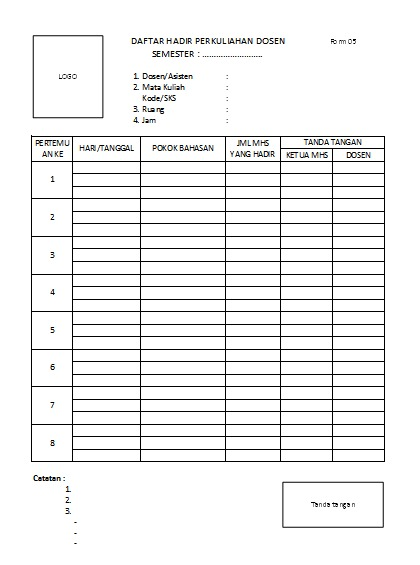
\includegraphics[width=0.7\textwidth]{gambar/form05-gambaran}
	\caption{Form 05}
\end{figure}

\begin{figure}[h!]
	\centering
	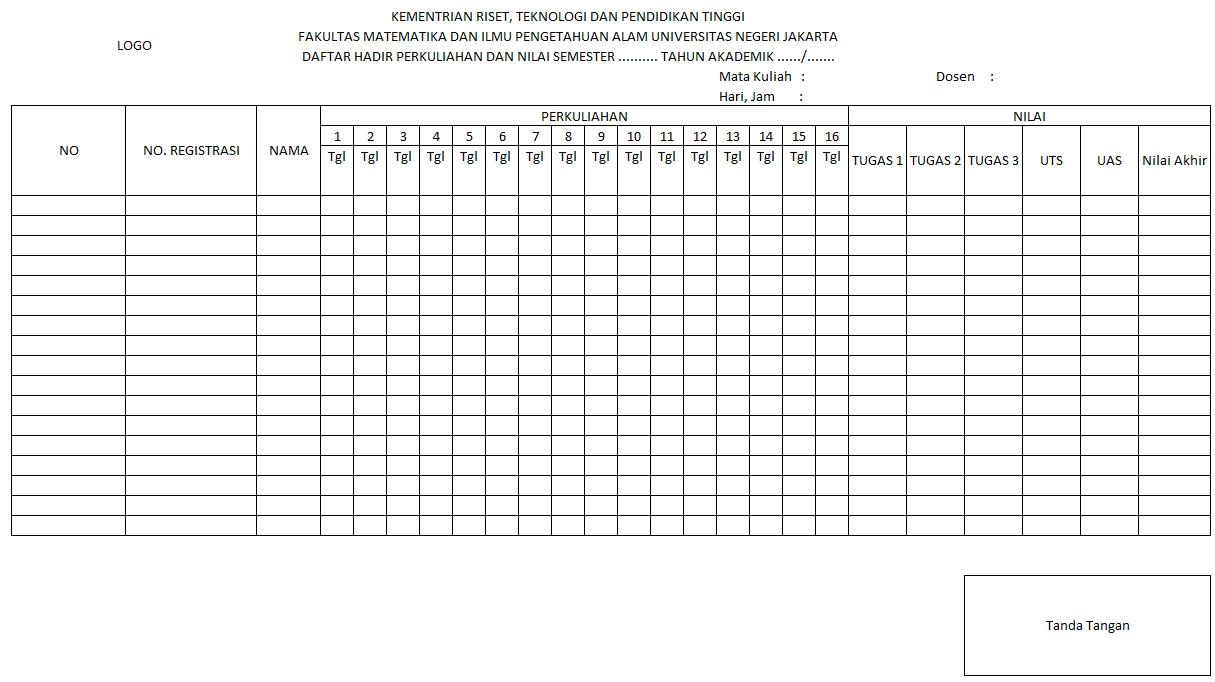
\includegraphics[width=0.7\textwidth]{gambar/form06-gambaran}
	\caption{Form 06}
\end{figure}

	Evaluasi form 05 dan 06 dilakukan tiga kali setiap semester. evaluasi pertama dilakukan pada minggu pertama untuk melihat mulainya pelaksanaan kuliah pertemuan pertama. Evaluasi kedua dilakukan sebelum Ujian Tengah Semester untuk melihat apakah jumlah pertemuan yang dilakukan sesuai atau cukup untuk melaksanakan Ujian Tengah Semester. Evaluasi ketiga dilakukan pada minggu terakhir untuk melihat apakah jumlah pertemuan mencapai syarat minimal 80\%. Evaluasi ini dilakukan oleh Tim Penjamin Mutu program studi dan nantinya akan dilaporkan ke Gugus Penjamin Mutu.


\section{Sistem Informasi}
\subsection{Definisi Sistem}
	Sistem adalah kumpulan atau grup dari bagian atau komponen apapun, baik fisik ataupun non fisik yang saling berhubungan satu sama lain dan bekerja sama untuk mencapai satu tujuan tertentu \citep{Susanto2017}. Sebuah sistem mempunyai karakteristik atau sifat-sifat tertentu, yaitu mempunyai komponen-komponen, batas sistem, lingkungan luar sistem, penghubung, masukan, keluaran, pengolah, dan sasaran atau tujuan \citep{Ladjamudin2005}.

	Menurut \cite{Romney2009}, sistem adalah suatu rangkaian yang terdiri dari beberapa komponen yang saling berhubungan dan saling berinteraksi antara satu sama lain untuk mencapai tujuan. Sistem biasanya terbagi menjadi subsistem yang lebih kecil yang mendukung sistem yang lebih besar. Dari pengertian-pengertian diatas, dapat disimpulkan bahwa sistem adalah kumpulan dari komponen-komponen yang saling berhubungan dan berinteraksi satu sama lain dalam sebuah rangkaian untuk mencapai tujuan.

\subsection{Definisi Informasi}
	Informasi adalah data yang telah diolah ke dalam bentuk yang lebih berguna dan lebih berarti bagi penggunanya. Informasi merupakan salah satu sumber daya paling penting yang dimiliki oleh suatu organisasi. Menurut \cite{Susanto2017} definisi informasi adalah hasil pengolahan data yang memberikan arti dan manfaat. Alat pengolahan informasi dapat berupa komponen komputer, komponen non komputer, atau kombinasi keduanya \citep{Ladjamudin2005}.

	Tidak semua data dapat digunakan untuk mendapatkan informasi yang berkualitas, data tersebut harus memiliki karakteristik tertentu. Untuk mendapat informasi yang berkualitas dibutuhkan data-data yang memiliki karakteristik sebagai berikut \citep{Kroenke2009}:
\begin{enumerate}
	\item Akurat

	Data yang benar, lengkap, dan akurat dan dengan didasarkan pengolahan yang sesuai akan menghasilkan informasi yang berkualitas. Dalam bisnis untuk mengambil keputusan sangatlah membutuhkan data yang akurat. Penggunaan data yang tidak akurat sebagai dasar pengambilan keputusan dapat memberikan dampak yang tidak diinginkan.

	\item Tepat Waktu

	Ketepatan waktu pada suatu informasi memiliki pengaruh yang sangat besar. Maksud dari ketepatan waktu tersebut adalah data yang digunakan dapat tersedia setiap waktu untuk digunakan sesuai kebutuhannya. Mengolah dan menghasilkan data secara cepat dan tepat akan menghasilkan informasi yang berkualitas dan dapat dimanfaatkan dengan tepat.

 Tepat waktu dimaksudkan dengan ketersediaan data setiap waktu diperlukan untuk dapat digunakan untuk kebutuhan tertentu. Infomasi yang berkualitas didapatkan dari data yang dapat diolah dan dihasilkan dengan cepat dan tepat agar pemanfaatannya dapat digunakan dengan tepat. Contohnya, ketika membuat sebuah laporan bulanan pada sebuah instansi, data yang diproses haruslah data yang didapatkan dalam satu bulan dan laporan tersebut harus selesai dengan secepatnya karena akan menjadi pertimbangan manajemen perusahaan dalam membuat keputusan selanjutnya.

	\item Relevan

	Informasi harus didapatkan dari data yang relevan baik dalam konteks maupun subjek. Relevansi data berdasarkan konteks dimaksudkan pada penggunaan data harus sesuai dalam bidangnya. Contohnya, untuk karyawan dengan sistem \textit{payroll}, data jam kerja merupakan data yang relevan dengan pekerjaan karyawan \textit{payroll} tersebut. Namun, daftar data jam kerja tersebut menjadi tidak relevan secara kontekstual jika digunakan untuk karyawan yang tidak menggunakan sistem payroll.

	Relevansi data berdasarkan subjek dimaksudkan pada data yang diatur berdasarkan subjeknya. Contohnya, ketika sebuah instansi membutuhkan data penawaran kredit oleh beberapa bank, maka data suku bunga merupakan data yang relevan berdasarkan subjek bank tersebut.

	\item Cukup

	Data yang cukup juga sangat berpengaruh dengan kualitas informasi yang dihasilkan. Kecukupan data dimaksudkan dengan ketersediaan data yang memenuhi keperluan dan tidak berlebihan dalam mengolah data tersebut menjadi informasi.

	\item Sebanding dengan biaya

	Memperoleh data tidaklah gratis. Ada biaya dalam melakukan pengolahan sebuah data termasuk memelihara sistem pengolah data, membayar gaji karyawan yang mengolah data, dan lain sebagainya. Atas dasar hal tersebut, data harus digunakan dengan bijak sehingga informasi yang dihasilkan dapat mengimbangi biaya yang dikeluarkan dalam mengolah data tersebut menjadi informasi.
\end{enumerate}

\subsection{Definisi Sistem Informasi}
	Sistem informasi adalah sebuah sistem dalam suatu keorganisasian yang mempertemukan kebutuhan pengelolaan, mendukung operasi, bersifat manajerial, dan kegiatan strategi dari suatu organisasi dan menyediakan pihak luar tertentu dengan laporan-laporan yang dibutuhkan \citep{Hutahaean2015}. Sistem informasi merupakan gabungan dari serangkaian komponen yang dapat berupa manusia, prosedur, data, dan teknologi yang digunakan untuk menghasilkan informasi yang bernilai sebagai dasar pengambilan keputusan.

	Sistem informasi memiliki komponen-komponen penting yang berinteraksi satu sama lain dan bekerja sama untuk melakukan suatu proses. Berikut adalah komponen-komponen dalam sistem informasi \citep{Jogiyanto2005}:

\begin{enumerate}

	\item Input, komponen input menjelaskan bagaimana sistem memperoleh atau menyediakan data untuk diproses lebih lanjut.
	\item Process, komponen process menjelaskan bagaimana suatu data diproses sehingga dapat menghasilkan informasi yang lebih bernilai.
	\item Output, komponen output adalah komponen hasil dari proses yang telah dilakukan sebelumnya.
	\item Penyimpanan, komponen penyimpanan merupakan komponen kegiatan yang dilakukan untuk menyimpan dan memelihara data.
	\item Pengendalian, komponen pengendalian merupakan komponen yang menjamin sistem informasi dapat berjalan sesuai yang diharapkan dan merupakan komponen paling penting dalam suatu sistem informasi.
\end{enumerate}
	Berdasarkan teori-teori dan pendapat diatas, dapat disimpulkan bahwa sistem informasi merupakan sebuah sistem dalam suatu organisasi yang bersifat manajerial dengan berbagai komponen yang berinteraksi dan bekerja sama antara satu dengan yang lain yang digunakan untuk menghasilkan informasi yang berkualitas dan dapat menjadi dasar dari suatu pengambilan keputusan.

\section{Software Development Life Cycle (SDLC)}
Proses pengembangan sebuah perangkat lunak dan sistem informasi selalu dipengaruhi oleh beberapa metodologi pengembangan. Metodologi pengembangan perangkat lunak mengacu pada kerangka kerja yang digunakan untuk merencanakan, mengelola, dan mengendalikan proses pengembangan sebuah sistem informasi. Metodologi pengembangan perangkat lunak disebut sebagai siklus hidup pengembangan perangkat lunak atau biasa dikenal sebagai \textit{Software Development Life Cycle}. SDLC adalah proses yang menjelaskan metode dan strategi mendesain dan memelihara proyek perangkat lunak untuk memastikan tujuan, sasaran, fungsional, dan kebutuhan pengguna dapat tercapai \citep{Arora2016}.

Proses pada metodologi SDLC umumnya dibagi menjadi beberapa fase, yaitu \citep{Dora2013}:

\begin{enumerate}
	
	\item \textit{Requirement Analysis}

	\textit{Requrement Analysis} adalah fase pertama dalam SDLC. Tujuan dari \textit{requirement analysis} adalah mengetahui dan mendokumentasikan kebutuhan sebenarnya dari pengguna. Fokus dari \textit{requirement analysis} adalah mengetahui apa yang dibutuhkan dari sistem yang akan dibuat. Fase ini adalah fase paling penting dalam SDLC. Hasil dari \textit{requirement analysis} adalah deskripsi lengkap dan komprehensif dari kegiatan yang dilakukan perangkat lunak yang akan dikembangkan.

	\item \textit{Design}

	Fase desain adalah fase paling kreatif pada SDLC. Pada fase desain, spesifikasi kebutuhan yang ada diubah menjadi bentuk terstruktur atau terencana. Fase ini merupakan proses perencanaan dan \textit{problem solving} untuk mencari solusi dengan perangkat lunak. Hasil dari fase ini adalah dokumen desain dari perangkat lunak yang akan dikembangkan.

	\item \textit{Coding}

	Pada fase \textit{coding}, dokumen desain dari perangkat lunak diubah menjadi \textit{code} dengan menggunakan bahasa pemrogramman tertentu. Fase ini adalah fase \textit{login} dari SDLC. Hasil dari fase ini adalah kode program.

	\item \textit{Testing}

	Segera setelah fase \textit{coding}, \textit{testing} dilakukan untuk mengetahui hasil dari aplikasi yang telah dikembangkan. \textit{Testing} dibuat untuk mengetahui hasil asli dan hasil yang diharapkan. Fase ini adalah fase paling penting dan berpengaruh. \textit{Testing} yang efektif akan menghasilkan produk perangkat lunak dengan kualitas tinggi, akurat, dan hasil yang dapat diandalkan.

	\item \textit{Maintenance}

	Fase akhir dari SDLC, dimana perangkat lunak yang telah dikembangkan didistribusikan ke pengguna akhir untuk pemeliharaan dan menggunakan untuk pengoperasian seharusnya.
\end{enumerate}

	SDLC memiliki berbagai macam model seperti Waterfall, V model, Spiral, Iterative, Agile, Extreme Programming, Scrum, dan lain sebagainya. Model yang akan dipilih dalam penelitian ini adalah Spiral. 

\section{Model Spiral} 

\begin{figure}[H]
	\centering
	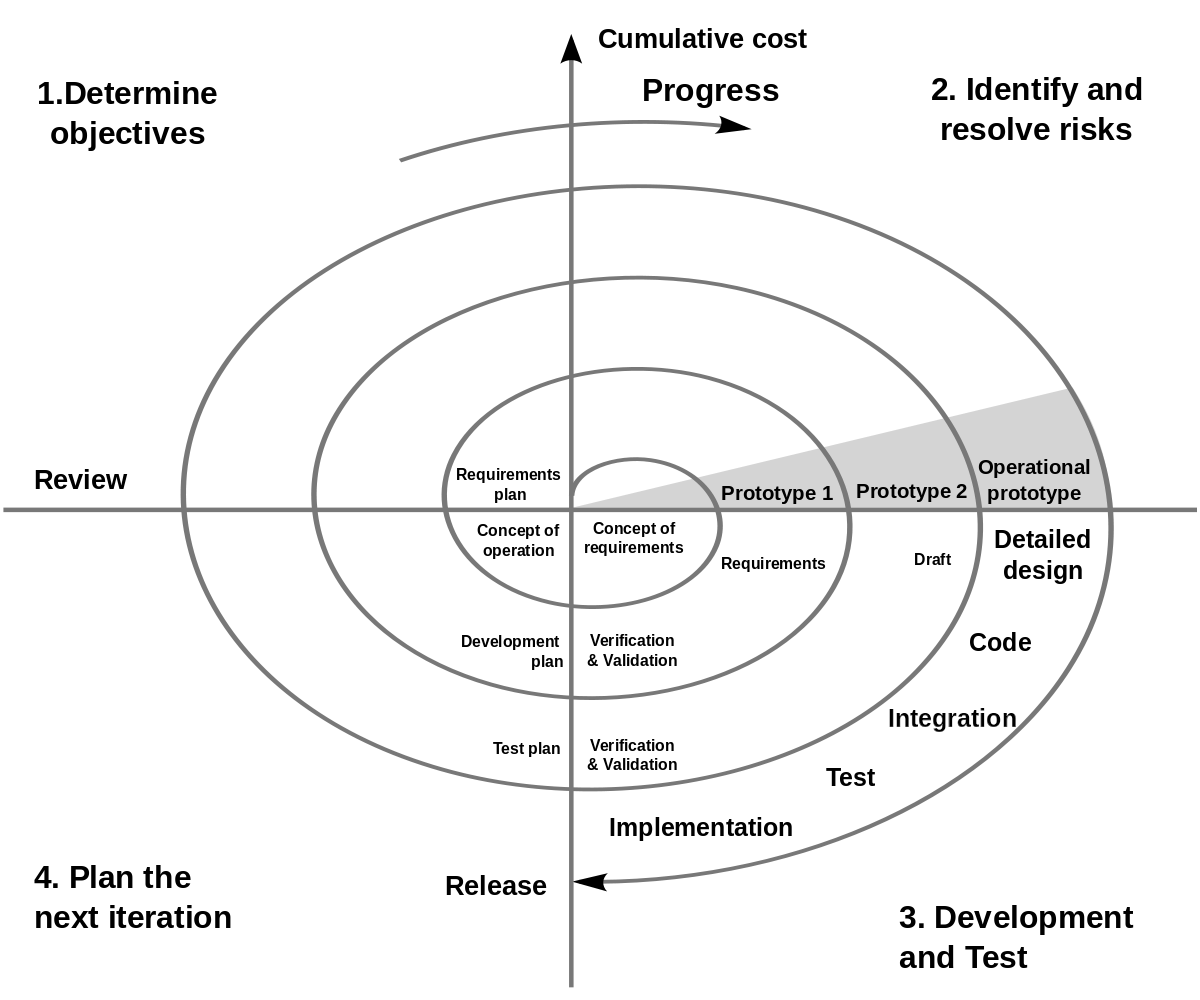
\includegraphics[width=0.7\textwidth]{gambar/Spiral}
	\caption{Model Spiral}
\end{figure}
Model Spiral adalah model SDLC yang menggabungkan proses model Iterative dengan elemen-elemen dari model Waterfall. Model Spiral berfokus pada analisis risiko dan meminimalkan risiko dari proyek. Hal tersebut dilakukan dengan cara membagi sebuah proyek menjadi beberapa bagian kecil sehingga mempermudah jika terdapat perubahan sekaligus melakukan evaluasi risiko dan mempertimbangkan kelanjutan proyek dalam prosesnya. Kemudahan dalam menerapkan model Spiral secara umum ditambah dengan kemudahan dalam melakukan perubahan sistem ketika ada fitur yang ingin ditambahkan ini adalah alasan penulis memilih model Spiral. Tidak seperti model lainnya yang selesai ketika perangkat lunak sudah diberikan ke pengguna, model spiral dapat digunakan sepanjang masa hidup digunakannya perangkat lunak tersebut. Oleh karena itu, iterasi pertama ada spiral dapat berupa konsep proyek yang dimulai pada pusat spiral dan berlanjut untuk beberapa iterasi hingga pengembangan konsep selesai. Jika konsep tersebut akan dibuat menjadi sebuah produk maka proses spiral dilanjutkan dan project pengembangan produk baru dimulai \citep{Pressman2010}. Fase-fase pada model Spiral dapat dideskripsikan sebagai berikut \citep{Alshamrani2015}: 

\begin{enumerate}

	\item Perencanaan

	Fase ini meliputi pemahaman dari kebutuhan sistem dengan melakukan komunikasi yang berkesinambungan antara pengguna dan sistem analis. Pada fase ini ditentukan tujuan yang akan dicapai pada iterasi yang akan berjalan.

	\item Analisis risiko
	
	Dalam fase ini dilakukan sebuah proses untuk mengidentifikasikan risiko yang dapat muncul dan solusi-solusi yang dapat dilakukan. Pada akhir fase ini menghasilkan sebuah prototipe.

	\item Pengembangan

	Pada fase ini program atau perangkat lunak dihasilkan sekaligus dengan dilakukannya pengujian.

	\item Evaluasi

	Fase ini memungkinkan pengguna untuk mengevaluasi hasil dari iterasi proyek sebelum dilanjutkan ke spiral selanjutnya. Pada fase ini dilakukan perencanaan iterasi selanjutnya berdasarkan dengan iterasi yang telah dilakukan.

\end{enumerate}


\section{\textit{Unified Modeling Language} (UML)}
	Menurut Windu dan Grace (2013) dalam jurnal \cite{Suendri2018} \textit{Unified Modeling Language} atau UML adalah bahasa spesifikasi standar yang biasa dipergunakan untuk mendokumentasikan, menspesifikasikan dan membangun perangkat lunak. UML merupakan sebuah metodologi dalam mengembangkan sistem berorientasi objek dan juga merupakan alat untuk mendukung pengembangan sistem.

	Saat ini UML telah menjadi standar bahasa visual yang digunakan untuk memodelkan sistem yang berorientasi objek. Fungsi dari UML adalah untuk melakukan pemodelan sehingga penggunaan dari UML sendiri tidak terbatas pada metodologi tertentu, meskipun pada kenyataannya UML paling banyak digunakan untuk metodologi berorientasi objek.

	Terdapat beberapa jenis diagram UML dan pada penelitian ini akan dibahas beberapa diantarana, yaitu:
\begin{enumerate}

	\item \textit{Use Case Diagram}

	\textit{Use case diagram} adalah diagram UML yang menggambarkan hal-hal apa saja yang dapat dilakukan oleh aktor atau pengguna dalam sistem yang dibuat. Aktor yang dimaksud di dalam \textit{Use Case Diagram} dapat berupa user, sistem internal, atau bahkan sistem eksternal yang dihubungkan dengan sistem yang dibuat. Simbol-simbol yang ada pada use case diagram dapat dilihat pada tabel \ref{tab:usecase}.

\begin{table}[h!]
\centering
\caption{Simbol-Simbol Pada \textit{Use Case Diagram}}
\label{tab:usecase}
\begin{tabular} { |>{\centering\arraybackslash}p{5cm}|p{6cm}| }
	\hline
	\textbf{Simbol} & \multicolumn{1}{>{\centering\arraybackslash}p{6cm}|}{\textbf{Deskripsi}} \\ 
	\hline
	\raisebox{-\totalheight}{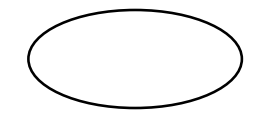
\includegraphics[scale=0.3]{gambar/usecase_usecase}}
	&
		\textit{Use case} adalah langkah atau tindakan yang dapat dilakukan di dalam sistem.
	\\
	\hline
	\raisebox{-\totalheight}{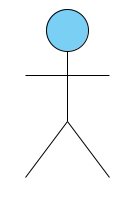
\includegraphics[scale=0.3]{gambar/actor_usecase}}
	&
		Aktor merupakan sebuah abstraksi dari pengguna atau peran yang lain yang terlibat dan berinteraksi dengan sistem.
	\\
	\hline
	\raisebox{-\totalheight}{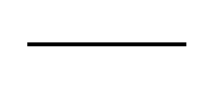
\includegraphics[scale=0.3]{gambar/asosiasi_usecase}}
	&
		Asosiasi adalah hubungan antara aktor dan \textit{use case} yang menggambarkan hubungan interaksi langsung antara keduanya.
	\\
	\hline
	\raisebox{-\totalheight}{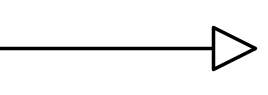
\includegraphics[scale=0.3]{gambar/generalisasi_usecase}}
	&
		Generalisasi adalah hubungan antara aktor yang menggambarkan kesamaan perilaku objek induk dengan objek anak.
	\\
	\hline
	\raisebox{-\totalheight}{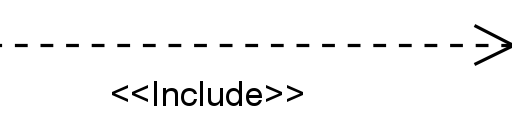
\includegraphics[scale=0.3]{gambar/include_usecase}}
	&
		\textit{Include} adalah hubungan antara \textit{use case} yang menggambarkan kebutuhan suatu \textit{use case} untuk dilanjutkan dengan \textit{use case} lain.
	\\
	\hline
	\raisebox{-\totalheight}{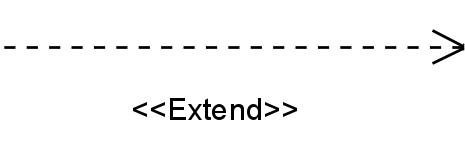
\includegraphics[scale=0.3]{gambar/extend_usecase}}
	&
		\textit{Extend} adalah hubungan antara \textit{use case} yang menggambarkan kemungkinan suatu \textit{use case} untuk dilanjutkan dengan \textit{use case} lain.
	\\
	\hline
\end{tabular}
\end{table}

	\item \textit{Class Diagram}

\textit{Class diagram} adalah sebuah diagram yang digunakan untuk menggambarkan kelas, atribut-atribut kelas, dan hubungan antar setiap kelas. Menurut Whitten dalam jurnal \cite{Suendri2018} kelas adalah suatu set objek yang memiliki atribut dan perilaku yang sama. Hubungan antar kelas dalam \textit{class diagram} memiliki keterangan yang biasa disebut dengan \textit{Multiplicity} atau \textit{Cardinality}. Ada beberapa jenis \textit{Multiplicity} sebagaimana digambarkan pada tabel \ref{tab:multiplicitybab2}. Simbol-simbol yang ada pada \textit{class diagram} dapat dilihat pada tabel \ref{tab:classdiagram}.

\begin{table}[h!]
\centering
\caption{\textit{Multiplicity} atau \textit{Cardinality} pada \textit{Class Diagram}}
\label{tab:multiplicitybab2}
\begin{tabular} { |>{\centering\arraybackslash}p{4cm}|p{5cm}| }
	\hline
	\textbf{\textit{Multiplicity}} & \multicolumn{1}{>{\centering\arraybackslash}p{6cm}|}{\textbf{Deskripsi Hubungan}} \\ 
	\hline

	1
	&
		Satu dan hanya satu.
	\\
	\hline
	0..*
	&
		Boleh tidak ada atau ada.
	\\
	\hline
	0..1
	&
		Boleh tidak ada atau hanya satu.
	\\
	\hline
	1..*
	&
		Harus ada dan boleh lebih dari satu.
	\\
	\hline
	n..m
	&
		Batasan jarak antara n dan m. Minimal n dan maksimal m.
	\\
	\hline
\end{tabular}
\end{table}

\begin{table}[h!]
\centering
\caption{Simbol-Simbol Pada \textit{Class Diagram}}
\label{tab:classdiagram}
\begin{tabular} { |>{\centering\arraybackslash}p{5cm}|p{6cm}| }
	\hline
	\textbf{Simbol} & \multicolumn{1}{>{\centering\arraybackslash}p{6cm}|}{\textbf{Deskripsi}} \\
	\hline
	\raisebox{-\totalheight}{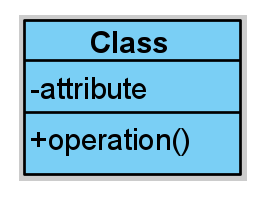
\includegraphics[scale=0.3]{gambar/classdiagram_kelas}}
	&
		Kelas merupakan elemen dan interaksi utama pada aplikasi.
	\\
	\hline
	\raisebox{-\totalheight}{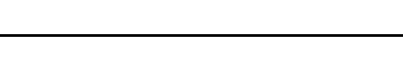
\includegraphics[scale=0.3]{gambar/classdiagram_asosiasi}}
	&
		Asosiasi adalah hubungan atau relasi umum antara kelas yang disertai dengan \textit{multiplicity}.
	\\
	\hline
	\raisebox{-\totalheight}{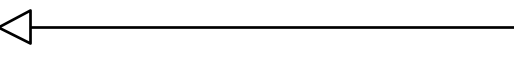
\includegraphics[scale=0.3]{gambar/classdiagram_generalisasi}}
	&
		Generalisasi adalah hubungan antara kelas yang menjelaskan bahwa suatu kelas merupakan \textit{superclass} dari kelas yang lain.
	\\
	\hline
	\raisebox{-\totalheight}{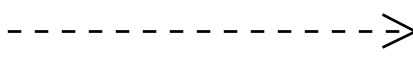
\includegraphics[scale=0.3]{gambar/classdiagram_depedensi}}
	&
		Generalisasi adalah hubungan antara kelas yang menggambarkan kesamaan perilaku \emph{superclass} dan \emph{subclass}
	\\
	\hline
	\raisebox{-\totalheight}{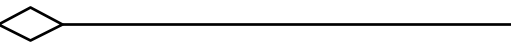
\includegraphics[scale=0.3]{gambar/classdiagram_agregat}}
	&
		Agregasi adalah hubungan atau relasi antar kelas yang bermakna semua objek kelas merupakan bagian dari kelas lain.
	\\
	\hline
	
\end{tabular}
\end{table}

	\item \textit{Activity Diagram}

	\textit{Activity diagram} adalah diagram yang digunakan untuk menggambarkan proses jalannya suatu aktivitas atau kegiatan yang dapat dilakukan dalam sebuah sistem. \textit{Activity diagram} biasanya menggambarkan bagaimana masing-masing kegiatan dimulai, keputusan yang mungkin terjadi di dalam kegiatan tersebut, hingga berakhirnya kegiatan yang dilakukan. \textit{Activity diagram} dapat menggambarkan lebih dari satu proses aksi dalam waktu bersamaan. Menurut Haviluddin dalam jurnal \cite{Suendri2018} \textit{Activity diagram} adalah aktivitas-aktivitas, objek, \textit{state}, transisi \textit{state}, dan \textit{event}. Dengan kata lain kegiatan diagram alur kerja menggambarkan perilaku sistem untuk aktivitas. Simbol-simbol yang digunakan pada activity diagram dapat dilihat pada tabel \ref{tab:activitydiagram}.

\begin{table}[h!]
\centering
\caption{Simbol-Simbol Pada \textit{Activity Diagram}}
\label{tab:activitydiagram}
\begin{tabular} { |>{\centering\arraybackslash}p{5cm}|p{6cm}| }
	\hline
	\textbf{Simbol} & \multicolumn{1}{>{\centering\arraybackslash}p{6cm}|}{\textbf{Deskripsi}} \\ 
	\hline
	\raisebox{-\totalheight}{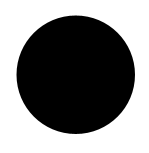
\includegraphics[scale=0.3]{gambar/activitydiagram_startpoint}}
	&
		\textit{Start Point} adalah poin dimulainya \textit{activity}.
	\\
	\hline
	\raisebox{-\totalheight}{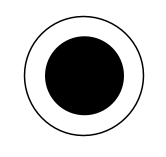
\includegraphics[scale=0.3]{gambar/activitydiagram_endpoint}}
	&
		\textit{End Point} adalah poin berakhirnya \textit{activity}.
	\\
	\hline
	\raisebox{-\totalheight}{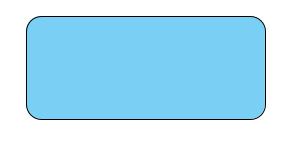
\includegraphics[scale=0.3]{gambar/activitydiagram_activity}}
	&
		\textit{Activity} menggambarkan suatu kegiatan atau proses bisnis.
	\\
	\hline
	\raisebox{-\totalheight}{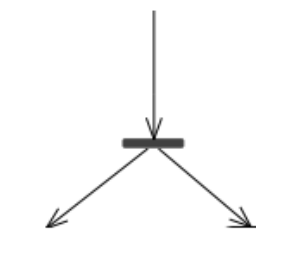
\includegraphics[scale=0.3]{gambar/activitydiagram_fork}}
	&
		\textit{Fork} adalah pembagian sebuah kegiatan menjadi lebih dari satu.
	\\
	\hline
	\raisebox{-\totalheight}{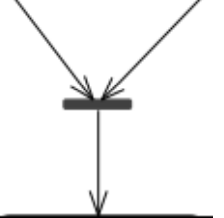
\includegraphics[scale=0.3]{gambar/activitydiagram_join}}
	&
		\textit{Join} adalah penggabungan kegiatan menjadi satu.
	\\
	\hline
	\raisebox{-\totalheight}{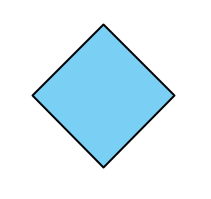
\includegraphics[scale=0.3]{gambar/activitydiagram_decisionnode}}
	&
		\textit{Decision Node} adalah pembagian sebuah kegiatan menjadi lebih dari satu berdasarkan keputusan yang diambil.
	\\
	\hline
	
\end{tabular}
\end{table}

\begin{comment}
	\item Sequence Diagram

	Sequence Diagram adalah salah satu tipe diagram interaksi yang menggambarkan bagaimana sekumpulan objek bekerja sama dan dalam urutan yang bagaimana. Menurut Haviluddin dalam jurnal \cite{Suendri2018} secara mudahnya sequence diagram adalah gambaran tahap demi tahap, termasuk kronologi (urutan) perubahan secara logis yang seharusnya dilakukan untuk menghasilkan sesuatu sesuai dengan use case diagram. Beberapa simbol-simbol yang digunakan dalam sequence diagram dapat dilihat pada tabel 

\begin{table}[h!]
\centering
\caption{Simbol-Simbol Pada Sequence Diagram}
\label{tab:sequencediagram}
\begin{tabular} { |>{\centering\arraybackslash}p{5cm}|p{6cm}| }
	\hline
	\textbf{Simbol} & \multicolumn{1}{>{\centering\arraybackslash}p{6cm}|}{\textbf{Deskripsi}} \\ 
	\hline
	\raisebox{-\totalheight}{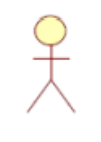
\includegraphics[scale=0.5]{gambar/sequencediagram_actor}}
	&
		Actor adalah sebuah abstraksi dari pengguna atau peran yang lain yang terlibat dan berinteraksi dengan sistem.
	\\
	\hline
	\raisebox{-\totalheight}{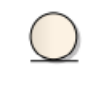
\includegraphics[scale=0.5]{gambar/sequencediagram_entityclass}}
	&
		Entity class adalah kelas yang berupa entitas-entitas utama sistem. Entity menggambarkan data pada sistem.
	\\
	\hline
	\raisebox{-\totalheight}{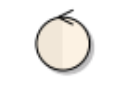
\includegraphics[scale=0.5]{gambar/sequencediagram_controlclass}}
	&
		Control class adalah kelas yang berisi logika-logika yang mengatur elemen-elemen pada sistem dan interaksinya.
	\\
	\hline
	\raisebox{-\totalheight}{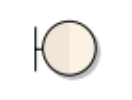
\includegraphics[scale=0.5]{gambar/sequencediagram_boundaryclass}}
	&
		Boundary class adalah kelas yang digunakan untuk memodelkan interaksi antara aktor dalam sistem.
	\\
	\hline
	\raisebox{-\totalheight}{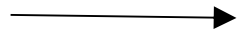
\includegraphics[scale=0.3]{gambar/sequencediagram_message}}
	&
		Message adalah pesan yang dikirimkan antara class.
	\\
	\hline
	\raisebox{-\totalheight}{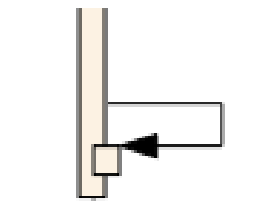
\includegraphics[scale=0.3]{gambar/sequencediagram_recursive}}
	&
		Recursive adalah pesan yang dikirimkan untuk class itu sendiri.
	\\
	\hline
	\raisebox{-\totalheight}{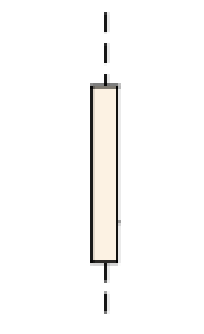
\includegraphics[scale=0.3]{gambar/sequencediagram_activation}}
	&
		Activation menggambarkan sebuah eksekusi operasi pada objek tersebut.
	\\
	\hline
	
\end{tabular}
\end{table}
\end{comment}

\end{enumerate}

\section{\textit{Entity Relationship Diagram}}

	\emph{Entity Relationship Diagram} (ERD) adalah sebuah tipe diagram struktural yang digunakan untuk mendesain \textit{database}. ERD memiliki banyak simbol dan penghubung yang digunakan untuk menggambarkan dua informasi penting, yaitu entitas utama dalam lingkup sistem dan hubungan antara masing-masing entitas yang ada. Menurut Simarmata(2010:67) dalam jurnal \cite{Fridayanthie2016} ERD adalah alat pemodelan data utama dan akan membantu mengorganisasi data dalam suatu proyek ke dalam entitas-entitas dan menentukan hubungan antar entitas. Sebuah ERD terdiri dari tiga komponen utama yaitu:

\begin{enumerate}

	\item \textit{Entity}

	\textit{Entity} atau entitas adalah sebuah benda atau konsep yang dapat didefinisikan di dalam sistem seperti Mahasiswa, Profil, Nilai, dan lain-lain. Notasi entitas biasanya dilambangkan dengan persegi panjang dengan nama dari entitas tersebut di atasnya dan berisi atribut dari entitas tersebut 

	\item \textit{Attribute}

	\textit{Attribute} adalah properti atau karakteristik dari suatu entitas. Sebuah atribut memiliki nama yang menjelaskan karakteristiknya dan tipe yang menjelaskan jenis dari karakteristik tersebut seperti \textit{varchar} atau \textit{int}. Sebagai contoh dalam entitas Mahasiswa terdapat atribut nama, nomor registrasi, alamat, dan lain-lain.

	\item \textit{Relationship}

	\textit{Relationship} dalam ERD adalah hubungan antara dua entitas yang menggambarkan bahwa kedua entitas tersebut memiliki suatu kaitan tertentu. Sebagai contoh seorang mahasiswa dapat mendaftarkan kelas yang ingin diikuti. \textit{Relationship} didefinisikan dengan menggunakan \textit{Foreign} \textit{Key} yang mengacu pada sebuah \textit{Primary Key}.
\end{enumerate}


\begin{figure}[H]
	\centering
	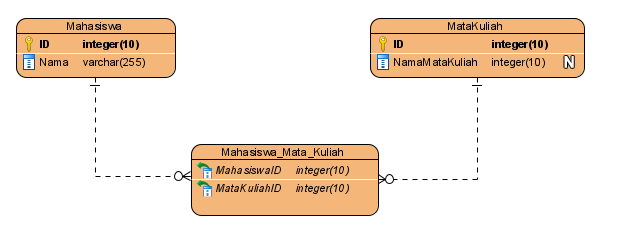
\includegraphics[width=1\textwidth]{gambar/contoh_erd}
	\caption{Contoh Sederhana ERD}
\end{figure}

\section{\textit{Database}}

	\textit{Database} merupakan sebuah kumpulan data-data yang terstruktur sehingga menjadi suatu informasi yang dapat dimanfaatkan. \textit{Database} terbentuk dari sekelompok data-data yang memiliki jenis atau sifat yang sama. Contohnya \textit{database} karyawan dapat berisi data-data berupa nama-nama, divisi-divisi, dan jabatan-jabatan karyawan.


	\textit{Database} adalah komponen yang paling penting dalam pembangunan sebuah sistem informasi, karena \textit{database} merupakan tempat untuk menyimpan dan mengelola seluruh data yang dimiliki. Data diatur sedemikian rupa sehingga tidak ada data yang terduplikasi agar data dapat diolah dengan tepat dan mudah untuk menghasilkan informasi.

	Menurut Susanto dalam jurnal \cite{Sudrajat2014} \textit{database} atau basis data adalah suatu kumpulan data terhubung (\textit{interrelated data}) yang disimpan secara bersama-sama dalam suatu media, tanpa mengatap satu sama lain atau tidak perlu kerangkapan data, data disimpan dengan cara-cara tertentu sehingga mudah untuk digunakan atau ditampilkan kembali. \textit{Database} dapat didefinisikan sebagai kumpulan data yang terintegrasi dan diatur sedemikian rupa sehingga data tersebut dapat dimanipulasi, diambil, dan dicari secara cepat \citep{Raharjo2011}.

	Untuk mengelola sebuah \textit{database} diperlukan sebuah perangkat lunak khusus yang disebut \textit{Database Management System} atau biasa disebut DBMS. DBMS adalah sebuah program yang digunakan untuk membuat, mendefinisikan, dan memelihara database. DBMS yang akan digunakan dan dibahas pada penelitian ini adalah MySQL yang juga merupakan salah satu DBMS yang paling banyak digunakan. MySQL merupakan sebuah DBMS \textit{Open Source} sehingga \textit{source code} dari MySQL dapat diakses secara umum dan dapat diunduh secara gratis. Menurut MySQL \textit{manual}, MySQL merupakan  perangkat lunak \textit{database} berbasis SQL (\textit{Structured Query Language}) yang dapat menangani sistem manajemen \textit{database} dan sistem manajemen \textit{database} relasional.

	Sebagai sebuah DBMS, MySQL memiliki beberapa fitur seperti:

\begin{enumerate}

	\item \textit{Multiplatform}

	MySQL tersedia pada berbagai platform umum seperti Windows, Linux, Unix, dan lain-lain.

	\item Dukungan SQL

	SQL sudah menjadi standar pada penggunaan \textit{database} relasional. Memiliki pengetahuan SQL akan sangat memudahkan penggunaan MySQL.

	\item Jaminan keamanan akses

	MySQL memberikan jaminan keamanan \textit{database} dengan beberapa kriteria pengaksesan.

	\item Cepat, handal, dan mudah digunakan

	MySQL termasuk sebagai \textit{database} \textit{server} yang handal, dapat menangani \textit{database} dengan ukuran besar dengan cepat, memiliki banyak fungsi pengaksesan, dan juga mudah digunakan.
\end{enumerate}

\section{\textit{Web Service}}

	\textit{Service} dalam dunia komputer adalah sebuah fungsionalitas dari program perangkat lunak yang dibuat untuk melayani kebutuhan dari program lain. Sebuah \textit{service} bertujuan untuk memungkinkan beberapa program lainnya untuk menggunakan \textit{service} tersebut dengan berbagai macam tujuan.  Menurut Wahli dkk dalam jurnal \cite{Fauziah2013} \textit{web sevice} merupakan suatu aplikasi modular yang bersifat mandiri dan dapat dipublikasikan, dialokasikan dan dipanggil melalui sebuah jaringan. Tujuan dari dibuatnya \textit{web service} adalah untuk membuat sebuah fungsionalitas yang dapat diakses melalui \textit{Internet Protocol} (IP) yang tidak bergantung pada platform dan bahasa pemrograman yang digunakan. \textit{Web service} dapat menjalankan fungsionalitas bisnis mulai dari yang sederhana seperti \textit{request-reply} hingga interaksi bisnis proses sepenuhnya. Untuk menjalankan proses yang rumit, sebuah \textit{web service} dapat bekerja sama atau mengandalkan \textit{web service} lain.

	\textit{Web service} dapat dibangun menggunakan beberapa bentuk arsitektur, salah satunya yang akan dibahas adalah \textit{Representational State Transfer}(REST). \textit{Web service} yang dibuat mengikuti arsitektur REST disebut RESTful \textit{Web Service}. Pada RESTful \textit{web} \textit{service}, \textit{server} menyediakan data atau sumber daya dan \textit{client} dapat mengakses data tersebut untuk digunakan. Setiap data atau \textit{resource} pada REST \textit{server} diidentifikasi oleh \textit{global id} yang merupakan URIs (\textit{Universal Resource Identifiers}). Pada umumnya data tersebut diberikan dalam format teks seperti JSON atau XML.

	Metode-metode HTTP yang biasa digunakan dalam RESTful \textit{Web Service} adalah sebagai berikut:

\begin{enumerate}

	\item \textit{Get}

		\textit{Get} adalah metode untuk membaca data.

	\item \textit{Post}

		\textit{Post} adalah metode untuk membuat data baru.

	\item \textit{Delete}

		\textit{Delete} adalah metode untuk menghapus data.

	\item \textit{Put}
		\textit{Put} adalah metode untuk memperbarui data yang sudah ada atau membuat data baru jika data belum ada.
\end{enumerate}

\section{\textit{Framework}}

	\textit{Framework} atau kerangka kerja adalah desain keseluruhan atau sebagian dari sistem yang berupa sebuah kumpulan kelas abstrak dan fungsi-fungsinya yang digunakan untuk mempermudah pengembangan sebuah perangkat lunak. Dengan menggunakan sebuah \textit{framework}, seorang \textit{developer} tidak perlu lagi mengimplementasikan fungsi-fungsi umum yang biasa digunakan karena sudah disediakan oleh \textit{framework} yang digunakan sehingga \textit{developer} hanya perlu menyesuaikan dengan kebutuhan dari program yang akan dibuat. \textit{Framework} dalam pembuatan \textit{website} umumnya terdapat dua jenis, yaitu \textit{framework} untuk membuat tampilan pengguna atau \textit{frontend} dan \textit{framework} untuk membuat sisi \textit{server} atau \textit{backend}. Beberapa \textit{framework} juga dapat digunakan untuk membangun keseluruhan dari sebuah \textit{website} mulai dari \textit{frontend} hingga \textit{backend}. Beberapa \textit{framework} yang dapat digunakan untuk membuat \textit{frontend} adalah AngularJS, ReactJS, dan VueJS. Sedangkan untuk \textit{backend} dapat menggunakan CI, Laravel, dan ExpressJS. Pada penelitian ini, digunakan dua \textit{framework} untuk membuat \textit{frontend} dan \textit{backend}, yaitu VueJS dan Laravel.

\section{MVC}

		Konsep MVC adalah sebuah pola desain perangkat lunak yang biasa digunakan untuk membangun user interface yang memisahkan logika pada program yang dibuat menjadi tiga elemen yang saling berhubungan. Tiga elemen tersebut adalah:

\begin{enumerate}

	\item \textit{Model}

	\textit{Model} merupakan komponen yang digunakan untuk mendefinisikan data-data utama yang akan digunakan dan berhubungan langsung dengan \textit{database}. \textit{Model} berisi struktur dari data yang akan digunakan beserta fungsi-fungsi yang bertujuan untuk mengolah data tersebut.

	\item \textit{View}

	\textit{View} adalah komponen yang mengatur tampilan \textit{website} yang dilihat oleh pengguna. Pada komponen inilah bagan, tabel, dan berbagai bentuk tampilan diproses. Umumnya komponen \textit{view} berupa \textit{file} HTML. Pada Laravel komponen \textit{view} bisa menggunakan \textit{templating} \textit{engine} Blade atau bisa menggunakan \textit{framework} Vue.JS.

	\item \textit{Controller}

	\textit{Controller} adalah komponen yang berisi segala logika dan alur kerja dari sistem. \textit{Controller} mengubah input yang diterima dari pengguna dan menentukan perintah selanjutnya yang akan dilaksanakan oleh aplikasi.

\end{enumerate}

		
\begin{figure}[h!]
	\centering
	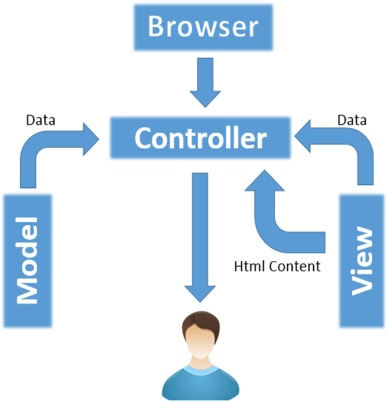
\includegraphics[width=0.5\textwidth]{gambar/mvc}
	\caption{Pola Desain MVC}
\end{figure}


	Selain dari memisahkan aplikasi menjadi tiga, konsep MVC juga mendefinisikan interaksi antara ketiganya. Ketika pengguna menggunakan aplikasi website, pengguna tersebut sedang berinteraksi dengan komponen view. Komponen view lalu menerima input dari pengguna dan meneruskan input tersebut ke controller. Controller lalu mengambil atau mengubah data pada model. Setelah mendapat data yang dibutuhkan Controller lalu mengembalikan data tersebut dan memperbarui view.




% Baris ini digunakan untuk membantu dalam melakukan sitasi
% Karena diapit dengan comment, maka baris ini akan diabaikan
% oleh compiler LaTeX.
\begin{comment}
bibliography{daftar-pustaka}
\end{comment}
